\documentclass[12pt]{extarticle}
\usepackage[utf8]{inputenc}
\usepackage{cite}
\usepackage{graphicx}
\usepackage{amssymb}
\usepackage[font=small,labelfont=bf]{caption}
\usepackage{subfig}
\usepackage{hyperref}

\title{Network Data Analysis - Assignment 1}
\author{Felipe M. Megale, 100806980}
\date{February 2022}

\begin{document}

\maketitle
\thispagestyle{empty}
\newpage
\tableofcontents
\thispagestyle{empty}

\section{Pre-processing data}
To complete the pre-processing of the original dataset, I used Pandas and Numpy. The first step for pre-processing the original file, after downloading it, was to remove all rows that had issues. Specifically speaking, this issue is not having either person name or ID. If either of these two information are missing, the row is removed from the original set. After removing those rows, I also removed those columns that did not have a label i.e., a question, and the two last questions that were further apart from the first 7. Furthermore, in order to have a more intelligible data set, I renamed the first column from \textit{"Unnamed: 0"} to \textit{"Name"}. Then, I isolated all questions and for each one of them, I created a new data set comprised of three attributes: \textit{"Name"}, \textit{"ID"}, \textit{"Question"}. This resulted in 7 new data sets, one for each question, which were saved as CSV files. The questions are:

\begin{itemize}
    \item "Which person you have hear of their voice or seen their faces?"
    \item "Which person you have met (in person+online) and exchange conversation?"
    \item "Which person you have collaborated with?"
    \item "Which person you have eye contact?"
    \item "Which peson you have eaten lunch with?"
    \item "Which person you have shared a ride?"
    \item "Which person you have taken at least two courses with?"
\end{itemize}

After having separated the questions, I processed the inputs of each question in each individual file. The reason for this was to simply adequate each person's input to comma-separated IDs by removing spaces and trailing characters such as commas and hyphens. Finally, for each of the 7 questions, I created 7 other files in the CSV format Gephi expects. For example, a line with the following values \textit{"1,2,3,4,5"} means that node 1 is connected to nodes 2, 3, 4 and 5.
\section{Analyses of 6 networks}
\subsection{Available networks}
For this assignment, out of the 7 available networks, the ones I chose to work with are networks 1 through 5, and 7.

Before describing each network individually, one characteristic all of them share is that the edges in all 7 graphs are unweighted for the same reason. The questions asked \textit{"which people?"}, meaning that for each person in the list, you only place an edge if the answer is yes. Because it is binary (edge or no edge), all graphs have unweighted edges. However, if we had a question asking \textit{"how many times?"}, then there is a possibility of having weighted edges. Also, Gephi does not render a node if its degree equals zero.

\subsubsection{Network 1}
\begin{figure}
    \centering
    \subfloat[\centering Network 1]{{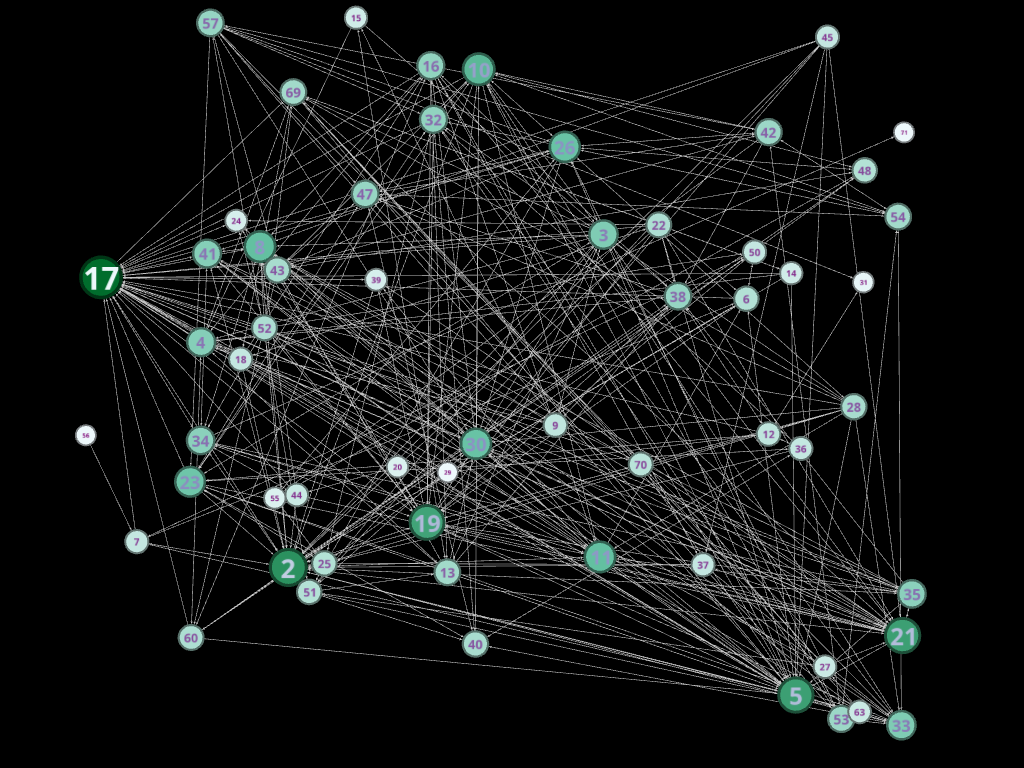
\includegraphics[width=0.45\textwidth]{img/net_0.png}}}
    \qquad
    \subfloat[\centering Network 2]{{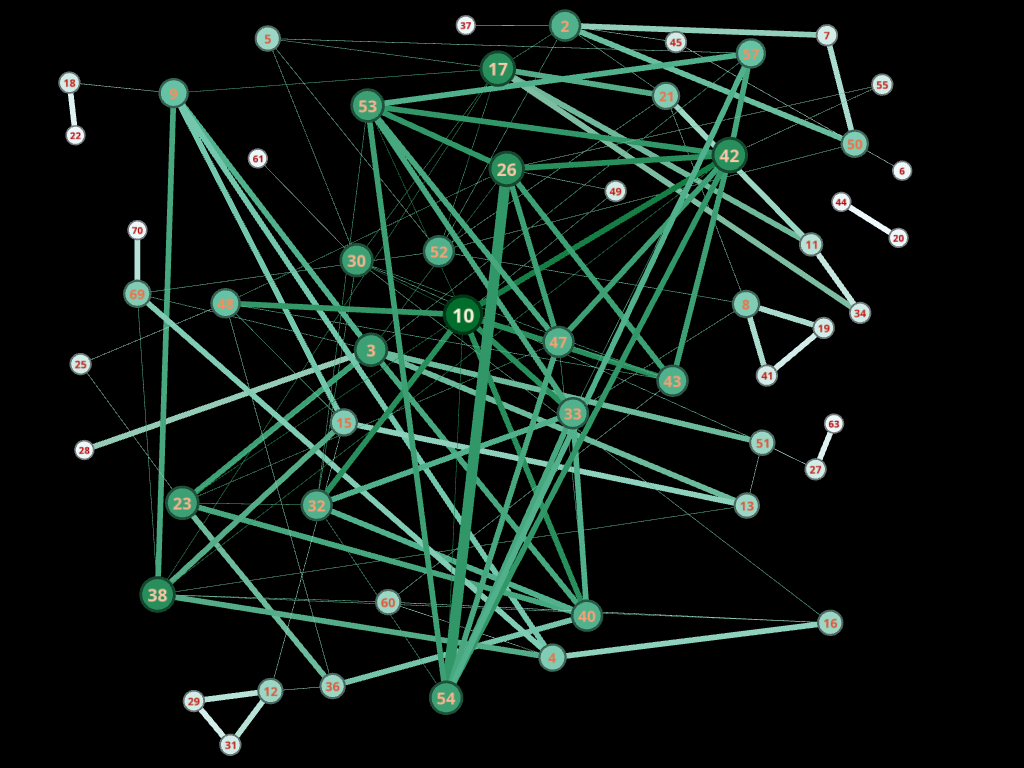
\includegraphics[width=0.45\textwidth]{img/net_1.png}}}
    \caption{Networks 1 \& 2}
    \label{fig:1}
\end{figure}

The first network asks the following question: \textit{"Which person you have hear of their voice or seen their faces?"}.

\textbf{Directed or undirected?} This network is an example of a directed graph. The reason for this is that in online conferences, it is not all participants who speak and/or have their computer cameras on. Therefore, I may see other people's faces and/or hear their voices, but they may not see or hear me.

\subsubsection{Network 2}
The second network asks the following question: \textit{"Which person you have met (in person+online) and exchange conversation?"}.

\textbf{Directed or undirected?} This network is an example of an undirected graph. In order to have a conversation, both parties must engage. If only one of them speak, there is no dialog. Therefore, is is not possible to exchange conversation.

\subsubsection{Network 3}
\begin{figure}
    \centering
    \subfloat[\centering Network 3]{{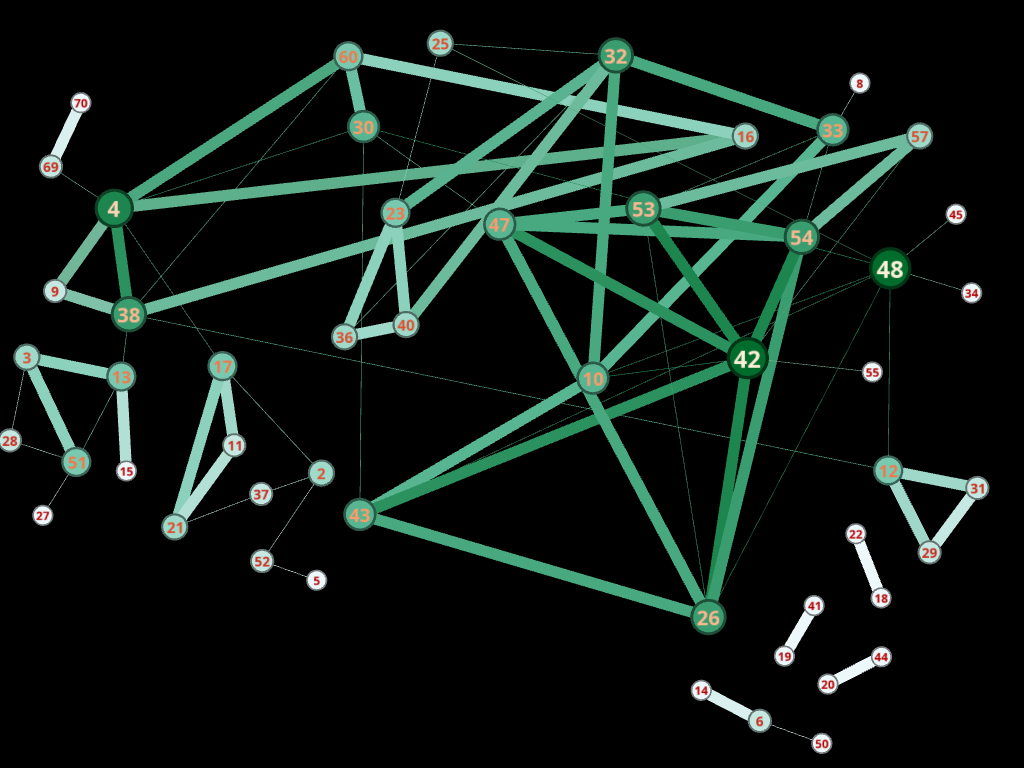
\includegraphics[width=0.45\textwidth]{img/net_2.png}}}
    \qquad
    \subfloat[\centering Network 4]{{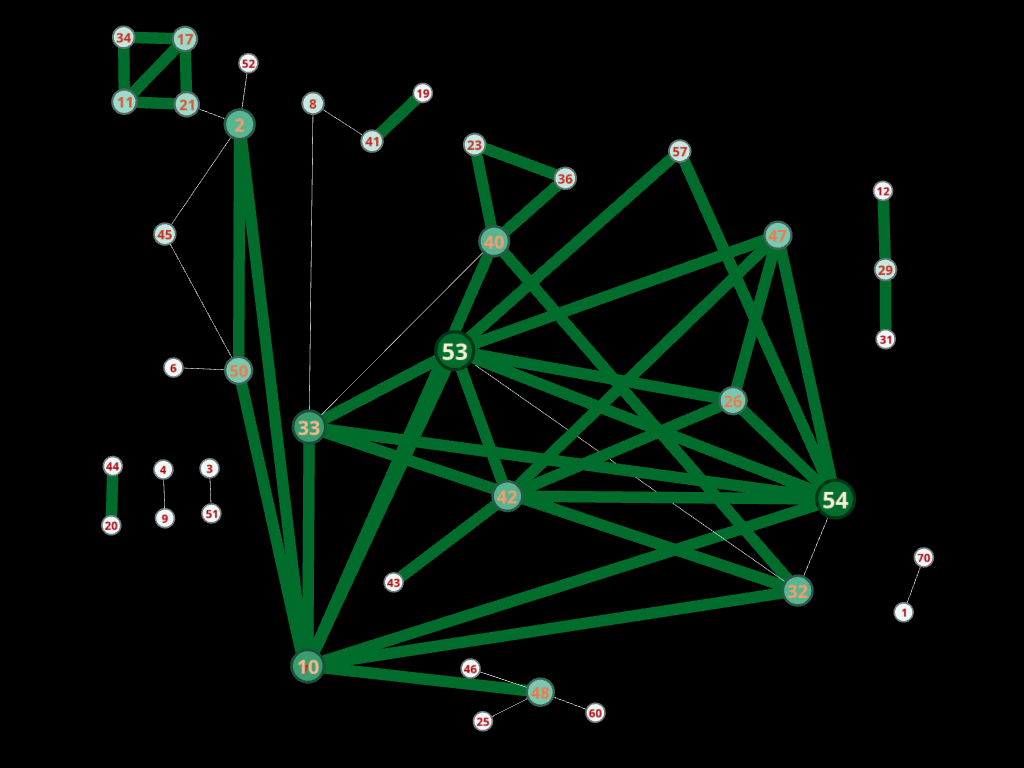
\includegraphics[width=0.45\textwidth]{img/net_3.png}}}
    \caption{Networks 3 \& 4}
    \label{fig:2}
\end{figure}

The third network asks the following question: \textit{"Which person you have collaborated with?"}.

\textbf{Directed or undirected?} This is an undirected graph because collaboration must be enforced by both parties. It has to be a mutual agreement.

\subsubsection{Network 4}
The fourth network asks the following question: \textit{"Which person you have eye contact?"}.

\textbf{Directed or undirected?} This network is undirected because in order to establish eye contact, two people must engage. There is no way for one person to look into someone else's eyes and not be looked back.

\subsubsection{Network 5}
\begin{figure}
    \centering
    \subfloat[\centering Network 5]{{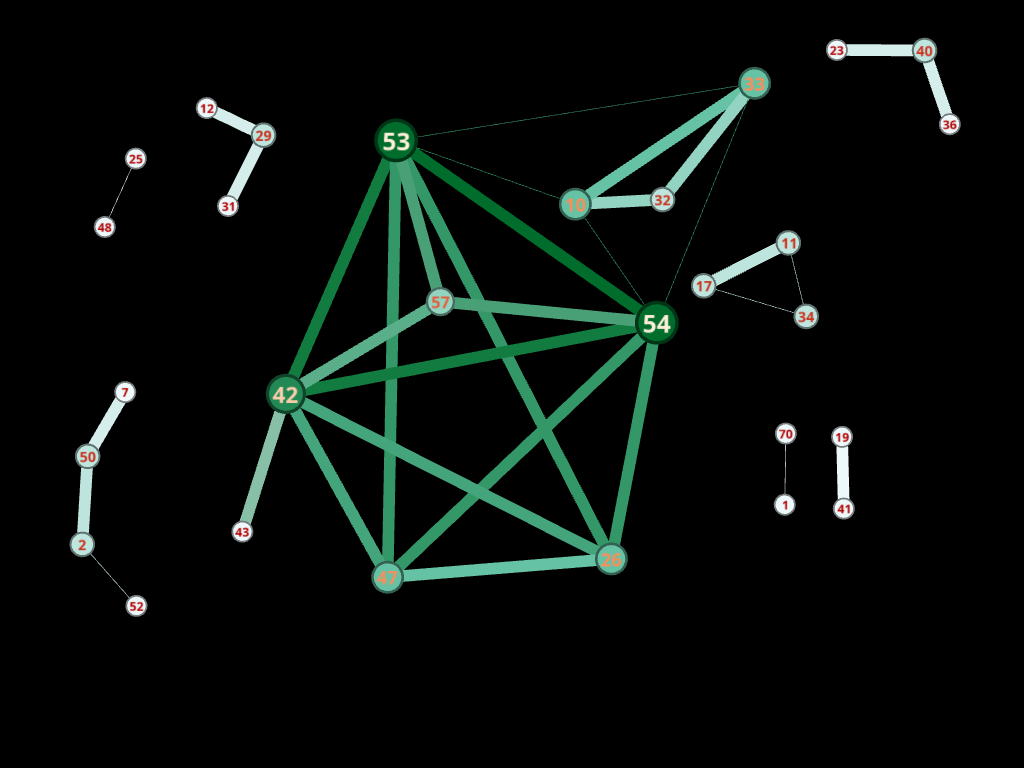
\includegraphics[width=0.45\textwidth]{img/net_4.png}}}
    \qquad
    \subfloat[\centering Network 7]{{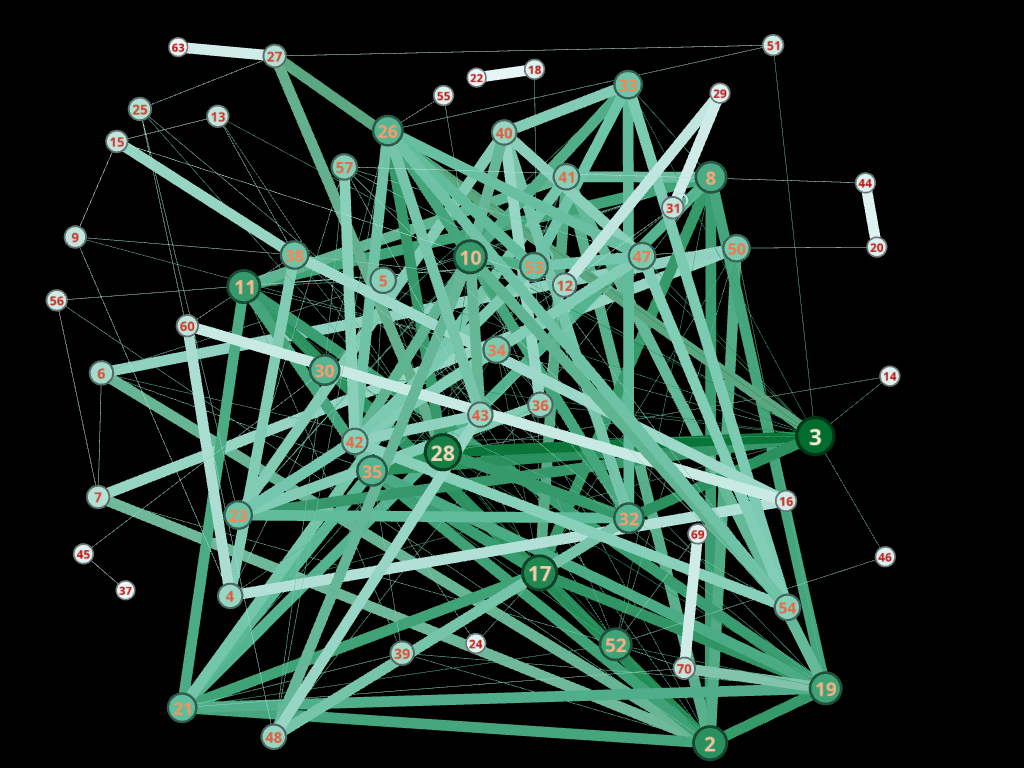
\includegraphics[width=0.45\textwidth]{img/net_6.png}}}
    \caption{Networks 5 \& 7}
    \label{fig:3}
\end{figure}

The fifth network asks the following question: \textit{"Which peson you have eaten lunch with?"}.

\textbf{Directed or undirected?} This is an undirected graph because eating lunch with another person implies that both people had to simultaneously engage in the activity.

\subsubsection{Network 7}
The seventh network asks the following question: \textit{"Which person you have taken at least two courses with?"}.

\textbf{Directed or undirected?} This network is an undirected graph because you cannot be simultaneously enrolled in a course another person has not and consider that as taking a course together. Also, the course must be taken in the same year.
\section{Metrics of 6 networks}
In this section I will present some statistics about the 6 chosen networks. The results will be presented in tables. It is also noteworthy to reiterate that Gephi does not display nodes if their degree is 0.

\begin{table}
    \centering
    \begin{tabular}{|c|c|c|c|c|c|c|c|}
        \hline
        \textbf{Metric} & \textbf{Net. 1} & \textbf{Net. 2} & \textbf{Net. 3} & \textbf{Net. 4} & \textbf{Net. 5} & \textbf{Net. 7} \\
        \hline
        Num. Nodes & 59 & 55 & 52 & 41 & 29 & 59 \\
        \hline
        Num. Edges & 427 & 124 & 80 & 54 & 34 & 216 \\
        \hline
        Density & 0.125 & 0.084 & 0.060 & 0.066 & 0.084 & 0.126 \\
        \hline
        Avg. Clust. Coef. & 0.375 & 0.412 & 0.482 & 0.583 & 0.620 & 0.542 \\
        \hline
        Num. Nodes SCC & 49 & - & - & - & - & - \\
        \hline
        Num. Nodes WCC & 58 & - & - & - & - & - \\
        \hline
        Num. Nodes CC & - & 52 & 42 & 20 & 10 & 59 \\
        \hline
        Avg. Path Len. SCC & 2.599 & - & - & - & - & - \\
        \hline
        Avg. Path Len. CC & - & 3.143 & 4.234 & 2.857 & 1.711 & 2.654 \\
        \hline
        Diameter of SCC & 7 & - & - & - & - & - \\
        \hline
        Diameter of CC & - & 7 & 11 & 6 & 4 & 6 \\
        \hline
    \end{tabular}
    \caption{Network statistics}
    \label{table:1}
\end{table}

\subsection{Number of nodes}
The number of nodes of each graph will be the amount of people who have at least one edge connecting them to another person.

\subsection{Number of edges}
The number of edges of each graph will be the amount of connections that exist between each person for each question.

\subsection{Edge density}
Graph density tells us how connected nodes are between each other. For undirected graphs, this metric can be calculated as
\begin{equation}
    D_{undirected} = \frac{2|E|}{|N|(|N|-1)}
    \label{equation:dir_density}
\end{equation}
and the density for directed graphs is defined as
\begin{equation}
    D_{directed} = \frac{|E|}{|N|(|N    |-1)}
    \label{equation:undir_density}
\end{equation}
where $E$ is the number of edges and $V$ is the number of nodes in the graph.

\subsection{Degree distribution}
The degree distribution of a graph allows us to grasp how deeply connected the nodes are. Figure \ref{fig:4} pictures the degree distributions for the 6 chosen networks.
\begin{figure}
    \centering
    \subfloat[\centering Network 1]{{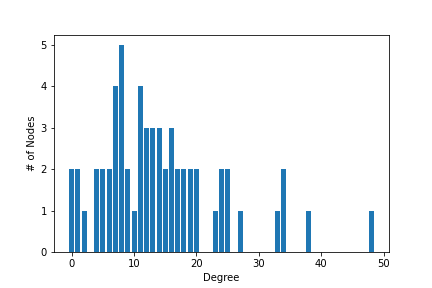
\includegraphics[width=0.45\textwidth]{img/net_0_degree_distribution.png}}}
    \qquad
    \subfloat[\centering Network 2]{{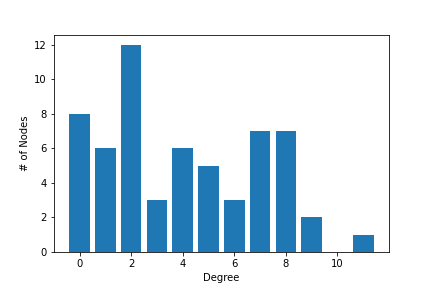
\includegraphics[width=0.45\textwidth]{img/net_1_degree_distribution.png}}}
    \qquad
    \subfloat[\centering Network 3]{{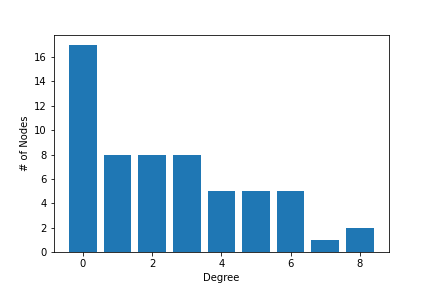
\includegraphics[width=0.45\textwidth]{img/net_2_degree_distribution.png}}}
    \qquad
    \subfloat[\centering Network 4]{{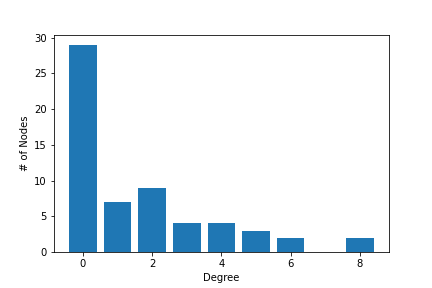
\includegraphics[width=0.45\textwidth]{img/net_3_degree_distribution.png}}}
    \qquad
    \subfloat[\centering Network 5]{{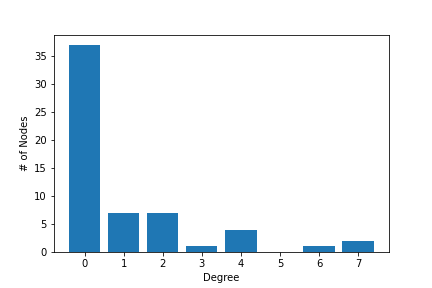
\includegraphics[width=0.45\textwidth]{img/net_4_degree_distribution.png}}}
    \qquad
    \subfloat[\centering Network 7]{{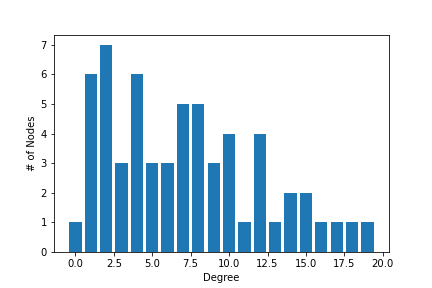
\includegraphics[width=0.45\textwidth]{img/net_6_degree_distribution.png}}}
    \caption{Degree distributions}
    \label{fig:4}
\end{figure}

\subsection{Average clustering coefficient}
The average clustering coefficient for a graph helps determine how transitive a relationship is. The clustering coefficient is defined as
\begin{equation}
    C_i = \frac{2e_i}{k_i(k_i-1)}
    \label{equation:clustering_coef}
\end{equation}
where $e_i$ is the number of edges between the neighbors of node $i$.

The average clustering coefficient of the graph is calculated as
\begin{equation}
    \left\langle C \right\rangle = \frac{1}{N}\sum_{i}^{N}C_i
    \label{equation:avg_clustering_coef}
\end{equation}
where $N$ is the number of nodes in the graph, and $C_i$ is the clustering coefficient of node $i$.

\subsection{Number of nodes in strongly connected component (SCC)}
The strongly connected component (SCC) metric can only be obtained from directed graphs. Since only the first network, then it is the only one that can provide this value. For networks 2 through 5, and 7, the values are from the connected components. Refer to table \ref{table:1} for the values.

\subsection{Number of nodes in weakly connected component (WCC)}
The weakly connected component (WCC) metric can only be obtained from directed graphs. Since only the first network, then it is the only one that can provide this value. For networks 2 through 5, and 7, the values are from the connected components. Refer to table \ref{table:1} for the values.

\subsection{Average path length in SCC}
The average path length metric indicates how far apart two nodes are from each other in the connected graph. In other words, how many jumps, in average, it takes to reach other nodes. For a directed graph, it is calculated as
\begin{equation}
    \left\langle d \right\rangle \equiv \frac{1}{2L_{max}}\sum_{i,j \neq i}d_{ij}
    \label{equation:dir_avg_path_len}
\end{equation}

For undirected graphs, it is calculated as
\begin{equation}
    \left\langle d \right\rangle \equiv \frac{1}{L_{max}}\sum_{i,j >  i}d_{ij}
    \label{equation:undir_avg_path_len}
\end{equation}

For networks 2 through 5, and 7, I calculated the average path length in the connected component because these networks are undirected graphs, thus not being possible to determine strongly connected components.

\subsection{Diameter of SCC}
This metric represents the maximum shortest distance between two nodes in a connected graph. It can be represented as
\begin{equation}
    diameter \equiv \max_{ij}d_{ij}
    \label{equation:diameter}
\end{equation}

For the first network, I collected the diameter of the strongly connected component. However, since all other networks are undirected graphs, I collected the diameter of the largest connected component.

\subsection{Community detection}
To detect communities in each of the chosen networks, I ran the Girvan--Newman algorithm, implemented in NetworkX. Figure \ref{fig:5} illustrates the communities in each network. The communities the algorithm found make sense, given that it ran by removing the edges with highest betweenness, separating the communities the edge held together. Also, by comparing with figures \ref{fig:1}, \ref{fig:2}, and \ref{fig:3}, we can see that the nodes with most connections between each other form a community the algorithm was able to find. Another interesting feature that the community detection algorithm allows us to perceive is that the more sparse the graph, the more communities we have. Figures \ref{fig:comm_3}, \ref{fig:comm_4}, and \ref{fig:comm_5} depict this behavior.
\begin{figure}[t]
    \centering
    \subfloat[\centering Network 1]{{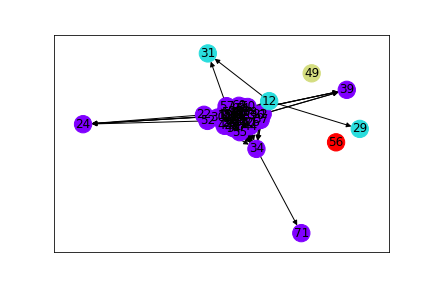
\includegraphics[width=0.45\textwidth]{img/net_0_communities.png}\label{fig:comm_1}}}
    \qquad
    \subfloat[\centering Network 2]{{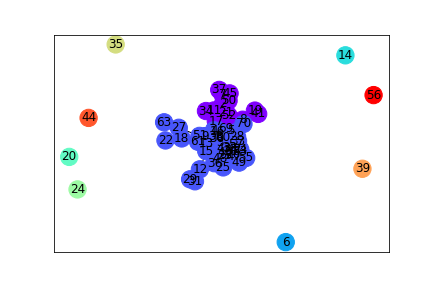
\includegraphics[width=0.45\textwidth]{img/net_1_communities.png}\label{fig:comm_2}}}
    \qquad
    \subfloat[\centering Network 3]{{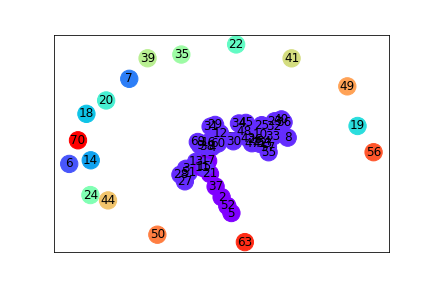
\includegraphics[width=0.45\textwidth]{img/net_2_communities.png}\label{fig:comm_3}}}
    \qquad
    \subfloat[\centering Network 4]{{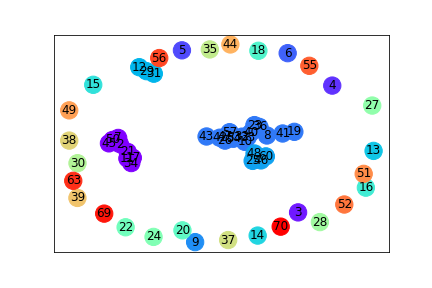
\includegraphics[width=0.45\textwidth]{img/net_3_communities.png}\label{fig:comm_4}}}
    \qquad
    \subfloat[\centering Network 5]{{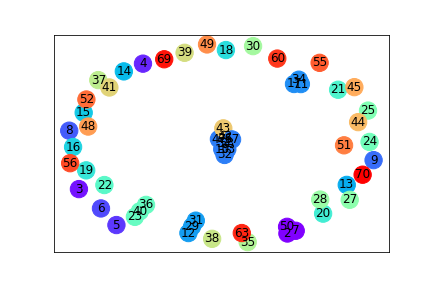
\includegraphics[width=0.45\textwidth]{img/net_4_communities.png}
    \label{fig:comm_5}}}
    \qquad
    \subfloat[\centering Network 7]{{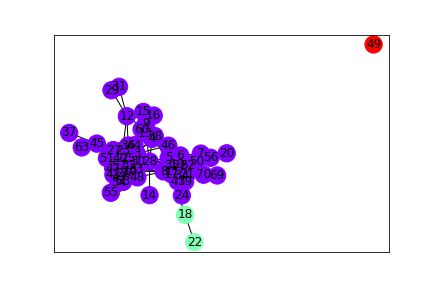
\includegraphics[width=0.45\textwidth]{img/net_6_communities.png}
    \label{fig:comm_7}}}
    \caption{Detected Communities}
    \label{fig:5}
\end{figure}

\subsection{Centrality Measures}
Centrality tries to determine which node is the most central in a graph. The four centrality measures will be used to determine which node is the most important in each network. The measures are in-degree, out-degree, betweenness, and closeness.

\subsubsection{Network 1}
For this network, in-degree and out-degree will be used to determine the two most central nodes. Because it is a directed graph, we can use these measures. The in-degree centrality of a node is calculated based on how many edges arrive in it. Similarly, the out-degree centrality of a node is calculated based on how many edges leave it. Table \ref{table:2} summarizes the two most people.
\begin{table}
    \centering
    \subfloat[\centering In-degree]{{
        \begin{tabular}{|c|c|c|}
            \hline
            \textbf{Rank} & \textbf{Person} & \textbf{Score} \\
            \hline
            1 & 17 & 0.576 \\
            \hline
            2 & 5 & 0.508 \\
            \hline
        \end{tabular}
        \label{table:net_0_in_deg}
    }}
    \qquad
    \subfloat[\centering Out-degree]{{
        \begin{tabular}{|c|c|c|}
            \hline
            \textbf{Rank} & \textbf{Person} & \textbf{Score} \\
            \hline
            1 & 10 & 0.271 \\
            \hline
            2 & 19 & 0.254 \\
            \hline
        \end{tabular}
        \label{table:net_0_out_deg}
    }}
    \caption{Network 1 centrality}
    \label{table:2}
\end{table}

\subsubsection{Network 2}
The centrality measures analyzed for this network were degree centrality and betweenness centrality. Degree centrality is similar to in-degree and out-degree centrality measures, except for the direction of the edges, which do not exist. The degree centrality measure for a node is defined by the amount of edges connected to it. Betweenness, on the other hand, is defined by the amount of shortest paths that go through a given node, and is calculated as follows
\begin{equation}
    C_B(i) = \sum_{j<k}\frac{g_{jk}(i)}{g_{jk}}
    \label{equation:betweenness_centrality}
\end{equation}
where $g_{jk}$ is the amount of shortest paths connecting nodes $j$ and $k$, and $g_{jk}(i)$ is the node currently being analyzed. Table \ref{table:3} summarizes the values found.
\begin{table}
    \centering
    \subfloat[\centering Degree]{{
        \begin{tabular}{|c|c|c|}
            \hline
            \textbf{Rank} & \textbf{Person} & \textbf{Score} \\
            \hline
            1 & 10 & 0.186 \\
            \hline
            2 & 42 & 0.152 \\
            \hline
        \end{tabular}
        \label{table:net_1_deg}
    }}
    \qquad
    \subfloat[\centering Betweenness]{{
        \begin{tabular}{|c|c|c|}
            \hline
            \textbf{Rank} & \textbf{Person} & \textbf{Score} \\
            \hline
            1 & 17 & 0.169 \\
            \hline
            2 & 30 & 0.131 \\
            \hline
        \end{tabular}
        \label{table:net_1_bet}
    }}
    \caption{Network 2 centrality}
    \label{table:3}
\end{table}

\subsubsection{Network 3}
The chosen centrality measures for this network were degree and closeness. Degree centrality has been previously defined. However, the closeness centrality measure is defined by the average length of shortest paths between a node and all other nodes in a graph. It can be calculated as
\begin{equation}
    C_C(i) = \left[\frac{1}{N-1}\sum_{j=1}^{N}d(i,j)\right]^{-1}
\end{equation}
where $N$ is the number of nodes in a graph, and $d(i,j)$ is the distance between nodes $i$ and $j$. Table \ref{table:4} summarizes the centrality results for this network.
\begin{table}
    \centering
    \subfloat[\centering Degree]{{
        \begin{tabular}{|c|c|c|}
            \hline
            \textbf{Rank} & \textbf{Person} & \textbf{Score} \\
            \hline
            1 & 48 & 0.137 \\
            \hline
            2 & 42 & 0.137 \\
            \hline
        \end{tabular}
        \label{table:net_2_deg}
    }}
    \qquad
    \subfloat[\centering Closeness]{{
        \begin{tabular}{|c|c|c|}
            \hline
            \textbf{Rank} & \textbf{Person} & \textbf{Score} \\
            \hline
            1 & 48 & 0.245 \\
            \hline
            2 & 30 & 0.243 \\
            \hline
        \end{tabular}
        \label{table:net_2_bet}
    }}
    \caption{Network 3 centrality}
    \label{table:4}
\end{table}

\subsubsection{Network 4}
The centrality measures chosen to analyze from this network were betweenness and closeness. These two measures have been previously defined. Table \ref{table:5} summarizes the values found.
\begin{table}
    \centering
    \subfloat[\centering Betweenness]{{
        \begin{tabular}{|c|c|c|}
            \hline
            \textbf{Rank} & \textbf{Person} & \textbf{Score} \\
            \hline
            1 & 10 & 0.039 \\
            \hline
            2 & 33 & 0.032 \\
            \hline
        \end{tabular}
        \label{table:net_3_bet}
    }}
    \qquad
    \subfloat[\centering Closeness]{{
        \begin{tabular}{|c|c|c|}
            \hline
            \textbf{Rank} & \textbf{Person} & \textbf{Score} \\
            \hline
            1 & 10 & 0.169 \\
            \hline
            2 & 33 & 0.165 \\
            \hline
        \end{tabular}
        \label{table:net_3_close}
    }}
    \caption{Network 4 centrality}
    \label{table:5}
\end{table}

\subsubsection{Network 5}
The centrality measures analyzed for this network were degree and betweenness centralities. These measures already have been introduced. Table \ref{table:6} summarizes the two most influential nodes of this network and their centrality score.
\begin{table}
    \centering
    \subfloat[\centering Degree]{{
        \begin{tabular}{|c|c|c|}
            \hline
            \textbf{Rank} & \textbf{Person} & \textbf{Score} \\
            \hline
            1 & 53 & 0.120 \\
            \hline
            2 & 54 & 0.120 \\
            \hline
        \end{tabular}
        \label{table:net_4_deg}
    }}
    \qquad
    \subfloat[\centering Betweenness]{{
        \begin{tabular}{|c|c|c|}
            \hline
            \textbf{Rank} & \textbf{Person} & \textbf{Score} \\
            \hline
            1 & 42 & 0.005 \\
            \hline
            2 & 53 & 0.004 \\
            \hline
        \end{tabular}
        \label{table:net_4_bet}
    }}
    \caption{Network 5 centrality}
    \label{table:6}
\end{table}

\subsubsection{Network 7}
The chosen centrality measures for network 7 were degree and closeness. I will refrain from going deeper into these concepts since they have already been introduced. Table \ref{table:7} summarizes the centrality findings for this network.
\begin{table}
    \centering
    \subfloat[\centering Degree]{{
        \begin{tabular}{|c|c|c|}
            \hline
            \textbf{Rank} & \textbf{Person} & \textbf{Score} \\
            \hline
            1 & 3 & 0.322 \\
            \hline
            2 & 28 & 0.305 \\
            \hline
        \end{tabular}
        \label{table:net_6_deg}
    }}
    \qquad
    \subfloat[\centering Closeness]{{
        \begin{tabular}{|c|c|c|}
            \hline
            \textbf{Rank} & \textbf{Person} & \textbf{Score} \\
            \hline
            1 & 28 & 0.543 \\
            \hline
            2 & 17 & 0.509 \\
            \hline
        \end{tabular}
        \label{table:net_6_close}
    }}
    \caption{Network 7 centrality}
    \label{table:7}
\end{table}

\section{Insights}
All the metrics previously calculated and visualized allow us to extract insightful knowledge about the networks that exist in our graduate program. Tackling the aspects of low degree distribution, low density and high number of communities, we can see that the questions \textit{"Which person you have collaborated with?"}, \textit{"Which person you have eye contact?"}, and \textit{"Which peson you have eaten lunch with?"} create the most sparse graphs. That may be due to the fact that most classes are still online and people haven't gotten the chance to interact with each other in a more meaningful way.

It is also interesting to notice unexpected behaviors on these sparse networks. Let us look at network 3 for example. It was one the three networks that were low in density and very sparse. However, the existing connected component was well connected. This means that despite existing many people who did not collaborate with their peers, the ones who did were thorough in doing it. However, because there were few edges in the whole graph, the average path length in the connected component was high. This is an indication that people collaborate together but they have their usual partners.

For network 5, which asks the question \textit{Which peson you have eaten lunch with?"}, we see that not many people have participated in this activity. Those who did, usually do frequently and there seems to be a closed group. Visualizing the network we are able to see that the connected component is almost a complete graph. This means that even though there are few connections in the graph, the ones that exist are meaningful.

Finally, discovering which nodes in each graph are more central is important. The reason for this is that knowing which people connect two or more components may contribute to how the people in these networks interact and collaborate with each other. Removing some of the key people from can result in disrupting an intricate collaboration network.
\section{Information Networks}

\subsection{Crawler Implementation}
\begin{lstlisting}[language=Python]
''' IMPORTS '''
# import HTML parser
from bs4 import BeautifulSoup

# import HTTP library
import requests

# import URL utility library
from urllib.parse import urlsplit

# import another URL utility library
import tldextract

# import sleep to prevent IP lockout
#     or intentional delays
from time import sleep

# import datetime to improve logging
from datetime import datetime

# python native queue data structure
from collections import deque

# native python json module, allows to serialize/deserialize json
import json
'''END IMPORTS'''

'''GLOBAL VARIABLES'''
# list of accepted domains
university_domains = ['uoit', 'ontariotechu'] 

# file extensions to be ignored
bad_file_extensions = ["mp4","mkv","pdf","docx","doc","mp3","wav","webp", "jpg", "png"]

# web page to begin traversing
INITIAL_URL = "https://ontariotechu.ca"

# this is a dictionary. each key is a URL and each value is a set of URLs that are referenced by the key
graph = {}

# this will be the queue of unvisited URLs
queue = deque()
'''END GLOBALS VARIABLES'''

''' BEGIN FUNCTIONS '''
# helper function to get formatted current datetime
def get_now():
    return datetime.now().strftime("%Y-%m-%d %H:%M:%S")

# lambda function to disregard all those hrefs that are not http or https pages
def filter_non_http(url):
    splitted_url = urlsplit(url)
    scheme = splitted_url.scheme
    if scheme not in ['http', 'https']:
        return False
    return True

# lambda function to filter off URLs with bad file extensions
def detect_bad_file_extensions(url):
    splitted_url = urlsplit(url)
    path = splitted_url.path

    for ext in bad_file_extensions:
        if ext in path:
            return False
    return True

# lambda function to 
def rstrip_url(url):
    splitted_url = urlsplit(url)
    scheme = splitted_url.scheme
    netloc = splitted_url.netloc
    path = splitted_url.path\
        .rstrip('/')\
        .replace('index.php', '')\
        .replace('index.html', '')\
        .replace('//','/')\
        .rstrip('/')
    new_url = f'{scheme}://{netloc}{path}'.rstrip('/')
    return new_url

# lambda function to convert uoit domain to ontariotechu
def uoit_to_ontariotechu(url):
    splitted_url = urlsplit(url)
    scheme = splitted_url.scheme
    netloc = splitted_url.netloc.replace('uoit','ontariotechu')
    path = splitted_url.path
    new_url = f'{scheme}://{netloc}{path}'.rstrip('/')
    return new_url

# key function for BFS. This expands the current node (URL)
def generate_children(url):
    try:
        # 1) sleep for 2 seconds to avoid ip blocking or slow down
        sleep(2)
        
        # 2) perform HTTP request to given URL
        print(get_now(), "GET HTTP request", url)
        r = requests.get(url)
        html_content = r.content

        # 3) parse HTML response to Python object
        soup = BeautifulSoup(html_content, "html.parser")

        # 4) get all anchor tags
        all_anchors = soup.find_all("a")
        
        # 5) get all hrefs from all anchors
        all_hrefs = []
        for anchor in all_anchors:
            try:
                all_hrefs.append(anchor['href'])
            except:
                pass

        # 6) filter off hrefs that are not in the UOIT or OTU domains
        university_hrefs = list(filter(lambda d: tldextract.extract(d).domain in university_domains, all_hrefs))

        # 7) filter off all URLs that are not http or https (e.g. mailto)
        university_hrefs = list(filter(filter_non_http, university_hrefs))

        # 8) filter off URLs that point to files
        university_hrefs = list(filter(detect_bad_file_extensions, university_hrefs))

        # 9) remove index.php or index.html, trailing slashes and double slashes
        university_hrefs = list(map(rstrip_url, university_hrefs))

        # 10) convert uoit domains to ontariotechu since uoit redirects to ontariotech
        university_hrefs = list(map(uoit_to_ontariotechu, university_hrefs))

        # 11) return all found children
        print(get_now(), 'Returning children...')
        return list(set(university_hrefs))
    except:
        return []

# bfs driver function
def bfs(url):
    print(get_now(), "Started BFS...")
    # 1) start by populating the queue with the initial node
    queue.append(url)

    # 2) while the queue isnt empty
    while len(queue) != 0:
        # 3) dequeue a node
        u = queue.popleft()

        # 4) get current nodes of the graph
        graph_keys = list(graph.keys())

        # 5) if the popped item is not a node in the graph
        if u not in graph_keys:
            print(get_now(), f'Generating children of {u}...')
            # 6) expand all nodes from current node
            children = generate_children(u)
            print(get_now(), 'Generated', len(children), 'children!')

            # 7) append to queue all chosen links in current web page
            for child in children:
                queue.append(child)
            
            # 8) add current node's adjacency list
            graph[u]=children
        # 9) if web page has been visited before, skip
        else:
            print(get_now(), f'Skipped {u} !')

    # 10) after traversing all web pages, dump graph to a json file for posterior processing and analytics
    print(get_now(), 'Writing adjacency list to file...')
    with open('bfs_adj_list.json', 'w') as f:
        f.write(json.dumps(graph))
    print(get_now(), 'Wrote adjacency list to file!')

''' END FUNCTIONS '''


# Python's main function
''' BEGIN MAIN '''
if __name__ == '__main__':
    program_begin = get_now()
    print(program_begin, "Starting BFS...")
    # start BFS from initial URL
    bfs(INITIAL_URL)
    program_end = get_now()
    print(program_end, "Program finished!")
    delta = program_end - program_begin
    print("Program took", delta, "to complete!")
''' END MAIN '''
\end{lstlisting}

\subsection{Code Explanation}
\subsubsection{Imports}
BeautifulSoup is responsible for converting the HTML string retrieved from the website into a serialized Python object. This allows for easy querying of all HTML tags and their attributes.

The \textit{requests} library is used to perform HTTP GET requests. The actual web page information is stored in the response's \textit{content} property.

From \textit{urllib} I imported the urlsplit function to easily split the URL into scheme, domain, and path. Query string parameters were ignored. In the same line of though, \textit{tldextract} was also used to easily extract the domain of the URL and change it in a lambda function from \textit{uoit} to \textit{ontariotechu} if it was the case.

The \textit{sleep} function from module \textit{time} was imported to force a 2-second wait before issuing the next HTTP request. This was done to avoid throttling, which would slow down the crawler's activity, and to prevent the domain from locking out my IP.

The \textit{datetime} function from module \textit{datetime} was imported to simply print out current date and time. The reason behind this was to improve logging quality.

The \textit{deque} class was imported from module \textit{collections} to ease the development of the BFS algorithm. It is a queue data structure and allows for queueing and dequeueing elements in it. It works as the queue of web pages that have not been visited yet.

Finally, the \textit{json} module was imported to dump the assembled graph into a JSON file. Because the crawling was a time-consuming task, having the graph readily available is important.

\subsubsection{Global Variables}
A \textit{university\_domains} list containing \textit{uoit} and \textit{ontariotechu} was used to hold the two University's known domains. It is employed on the filtering of URLs that point to outside of the University's network. This way I can keep crawl only the pages that belong and refer to the Ontario Tech University.

The \textit{bad\_file\_extensions} list holds a few of the common file extensions that may be present on a URL. It, too, is used to filter off web pages that would host files. Since they are not actual web pages, it makes no sense to go through them.

Simply, the \textit{INITIAL\_URL} is just a variable that is used to trigger the Breadth First Search Algorithm. It is passed in the main method as the starting node.

The \textit{graph} variable is a dictionary that will be the assembled graph. The keys will be the URLs and the adjacency list will be a set of URLs the node has hyperlinks to.

Finally, the \textit{queue} variable starts as an empty queue. This queue is used to hold the web pages that have yet to be visited.

\subsubsection{Functions}
The \textit{get\_now} function is a wrapper for the \textit{datetime} function. It's only purpose is to return a formatted string containing the current date and time, for logging purposes.

Next, the \textit{filter\_non\_http} function is a lambda function. It is used in a \textit{filter} list function to remove all URLs that are not HTTP or HTTPS schemes. An example of a URL that was removed was a \textit{mailto}.

The \textit{detect\_bad\_file\_extensions} function is another lambda filter function. It works by splitting the URL and grabbing its path - the path is everything that comes after the country (e.g. \textit{.ca}) - and searching for any of the aforementioned bad file extensions.

Following the list of helper functions, the \textit{rstrip\_url} is another lambda function. This one, on the other hand, is used in a list mapping. It works by splitting a URL and altering the path to remove trailing slashes, any files that are index files (HTML or PHP). This function then returns the stripped URL.

The next lambda function is called \textit{uoit\_ontariotechu}. The sole purpose of this function is to map all URLs that are in the UOIT domain to Ontario Tech University's domain. This avoids adding nodes to the graph that are different in name, but that point to the same content.

Next, the core of the BFS algorithm, is the \textit{generate\_children} function. It works by trying to perform an HTTP GET request. When the request fails by any reason, I say that no children were found, since no web page was collected. If the request does not fail, I collect the content (namely, the HTML page as a string), parse it with \textit{BeautifulSoup}, query all anchor HTML tags, then try to collect every href attribute from the anchors. Next, I process all hrefs using a series of mappings and filters. I first filter off those URLs that are not in the UOIT/Ontario Tech University domain. Then the remaining URLs are filtered to remove every scheme that is not HTTP not HTTPS. The remaining URLs are again filtered to remove those that host files. Next, I map the URLs to remove trailing slashes and index pages. Finally, the remaining set of URLs is mapped again, but this time to change all UOIT domains into Ontario Tech University domains. After this series of mappings and filters, the remaining URLs are put into a set, which in Python removes duplicates from any list, and returned. This finishes the execution of the \textit{generate\_children} function.

Lastly, the \textit{bfs} function is the actual implementation of the Breadth First Search algorithm. It starts by pushing to the queue the URL that was passed as a parameter. Then, until the queue is not empty, it dequeues a node that has not yet been visited and gets the current list of nodes in the graph. If the dequeued node is not in the list of nodes, expand the graph by generating the current node's children. Then, for each child of the current node, add it to the queue then add all children as the adjacency list of the current node in the graph. if the dequeued node is in the list of nodes in the graph, skip it to avoid performing unnecessary HTTP requests. When the queue is empty, the function dumps the assembled graph to a JSON file for persistent storage and avoid running the crawler every time the graph is needed.

\subsubsection{Main}
The main function in Python is used to call the \textit{bfs} function. It passes the \textit{INITIAL\_URL} as parameter. This function is the starting point of a Python program. It also calculates how long it took for the crawler to finish traversing all web pages in the Ontario Tech University's domain.

% Write about the proposed work touching the research gap you are addressing, novelty etc. When you are using some references, make sure you list them in the reference below and cite them in this section \cite{Linhart2014} \cite{Linhart2008}.

% And in the last paragraph write about the proposed deliverable aimed from this thesis  \cite{fractalwiki}.

% Proposed Guides: Dr./Mr./Ms Name of faculty, Professor/Associate/Assistant Professor, Department, Campus.  \nocite{higham1998handbook}


\bibliographystyle{plain}
\bibliography{M335}

\end{document}
